\NewsItem{Feuchtemessverfahren}

\begin{multicols}{2} 

%%======================================================================== Text Einfügen
{ \centering
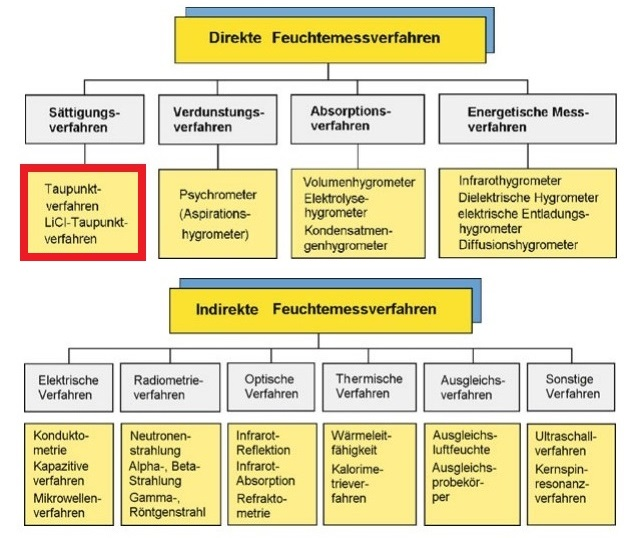
\includegraphics[width=\columnwidth]{graphics/verfahren.jpg}\\
\captionof{figure}{Direkte und indirekte Messverfahren \cite{Hesse2014}}
\label{dir_inddir_Messverf}
}
\vfill\columnbreak
Die Verfahren zur Feuchtemessung werden unterteilt in direkte und indirekte Methoden. Das direkte Feuchtemessverfahren trennt das Wasser direkt vom Feststoff. Das indirekte Verfahren misst Substanzeigenschaften, die durch den Wassergehalt messbar verändert werden, um danach über eine Kennlinie auf den Feuchtigkeitsgehalt zu schliessen. \cite{Hesse2014}\cite{Giessereilexikon}\\[0.5cm]
Die Luftfeuchtigkeit lässt sich mit verschiedenen Verfahren messen. MeteoSchweiz nutzt für die Temperatur- und Luftfeuchtemessung unter anderem das Instrument Thygan der Schweizer Firma Meteolabor AG, welches sehr genau und für extreme Witterungsbedingungen geeignet ist. Dieses Instrument nutzt das Verfahren mittels Taupunktspiegel, welches ein Sättigungsverfahren nutzt und somit zu den direkten Feuchtemessverfahren gehört. \cite{MeteoSchweiz2014}\\
\end{multicols}